\documentclass{article}
\usepackage{amsfonts} % if you want blackboard bold symbols e.g. for real numbers
\usepackage[margin=1.0in]{geometry}
\usepackage{graphicx} 
\usepackage{amsmath}
\usepackage{amssymb}
\usepackage{hyperref}
\hypersetup{
    colorlinks,
    citecolor=blue,
    filecolor=black,
    linkcolor=blue,
    urlcolor=black
}
\title{Vortex Sheet Evolution}
\author{Rajesh Venkatesan}
\date{}

\begin{document}
\maketitle
\section{Birkhoff-Rott Equation}
The complex potential at a point $z=x+iy$ due to a point vortex of strength $\Gamma$ (anti-clockwise being positive) located at $z_0=x_0+iy_0$ is given by,
\begin{equation}
w(z)=-\frac{i\Gamma}{2\pi} \log{(z-z_0)}
\end{equation}
If there are $2n+1$ number of vortices of equal strength $\Gamma$ located at $(0,0),(\pm \lambda,0),(\pm 2\lambda,0),...(\pm n\lambda,0)$, then the complex potential at the point $z$ is,
\begin{align*}
w(z)&=-\frac{i\Gamma}{2\pi}\left[\log{(z)}+\log{(z-\lambda)}+\log{(z+\lambda)}+\log{(z-2\lambda)}+\log{(z+2\lambda)}+...+\log{(z-n\lambda)}+\log{(z+n\lambda)}\right] \\
&= -\frac{i\Gamma}{2\pi}\log\left[z(z^2-\lambda^2)(z^2-2^2\lambda^2)(z^2-3^2\lambda^2)...(z^2-n^2\lambda^2)\right]\\
&=-\frac{i\Gamma}{2\pi} \log \left[z\left(1-\frac{z^2}{\lambda^2}\right)\left(1-\frac{z^2}{2\lambda^2}\right)...\left(1-\frac{z^2}{n^2\lambda^2}\right)\times \left(-1\right)^n\cdot\lambda^2\cdot 2^2 \lambda^2 ... n^2 \lambda^2\right] \\
&=-\frac{i\Gamma}{2\pi} \log \left[\frac{\pi z}{\lambda}\left(1-\frac{z^2}{\lambda^2}\right)\left(1-\frac{z^2}{2\lambda^2}\right)...\left(1-\frac{z^2}{n^2\lambda^2}\right)\right] +\frac{-i\Gamma}{2\pi} \log \left[ \left(-1\right)^n\cdot\frac{\lambda}{\pi}\cdot \lambda^2\cdot 2^2 \lambda^2 ... n^2 \lambda^2\right]\\
\end{align*}

Since the second term in the last equation is a constant, it can be neglected considering $w(z)$ is a potential. So,
\begin{align}
w(z)&=-\frac{i\Gamma}{2\pi} \log \left[\frac{\pi z}{\lambda}\left(1-\frac{z^2}{\lambda^2}\right)\left(1-\frac{z^2}{2\lambda^2}\right)...\left(1-\frac{z^2}{n^2\lambda^2}\right)\right]
\end{align}

Now letting $n\rightarrow \infty$, we have an infinite number of vortices located at $(0,0),(\pm \lambda,0),(\pm 2\lambda,0),...$ and the complex potential at $z$ is given by,

\begin{align}
w(z)=w(z)&=-\frac{i\Gamma}{2\pi} \log \left[\frac{\pi z}{\lambda}\prod_{n=1}^{\infty}\left(1-\frac{z^2}{n^2\lambda^2}\right)\right]
\end{align}
Using the infinite product expression for the sine function,
\begin{equation}
\sin x = x \prod_{n=1}^{\infty}\left(1-\frac{x^2}{n^2\pi^2}\right)
\end{equation}
We have,
\begin{align}
w(z)&= -\frac{i\Gamma}{2\pi} \log \sin \frac{\pi z}{\lambda}
\end{align}
Or,
\begin{align}
w(z)&=-\frac{i\Gamma}{2\pi} \log \sin \frac{\pi (z-z_0)}{\lambda} 
\end{align}

where $z_0$ is the location of one of the vortices and $\lambda$ is the spacing between vortices.

The velocity induced at the point $z_1=x_1+iy_1$ is then given by,
\begin{align*}
\frac{dw}{dz}\vline _{z=z_1}&=u-iv \\
&= -\frac{i \Gamma }{2 \pi} \frac{1}{\sin (\pi(z_1-z_0)/\lambda)} \cos \left(\frac{\pi(z_1-z_0)}{\lambda}\right) \cdot \frac{\pi}{\lambda} \\
&= -\frac{i\Gamma}{2\lambda} \cot{\frac{\pi(z_1-z_0)}{\lambda}}
\end{align*}

We need to seperate the real and imaginary parts to obtain the velocity components explicitly.
\begin{align*}
&=-\frac{i\Gamma}{2\lambda} \frac{\cos\pi[(x_1-x_0)+i(y_1-y_0)]/\lambda}{\sin\pi[(x_1-x_0)+i(y_1-y_0)]/\lambda} \\
&=-\frac{i\Gamma}{2\lambda} \frac{\cos(\pi(x_1-x_0)/\lambda)\cosh(\pi(y_1-y_0)/\lambda)-i\sin(\pi(x_1-x_0)/\lambda)\sinh(\pi(y_1-y_0)/\lambda)}{\sin(\pi(x_1-x_0)/\lambda)\cosh(\pi(y_1-y_0)/\lambda)+i\cos(\pi(x_1-x_0)/\lambda)\sinh(\pi(y_1-y_0)/\lambda)}
\end{align*}
Multiplying and dividing by the complex conjugate of the denominator, we get,
\begin{align*}
&= -\frac{i\Gamma}{2\lambda} \frac{\cos(\pi(x_1-x_0)/\lambda)\cosh(\pi(y_1-y_0)/\lambda)-i\sin(\pi(x_1-x_0)/\lambda)\sinh(\pi(y_1-y_0)/\lambda)}{\sin^2(\pi(x_1-x_0)/\lambda)\cosh^2(\pi(y_1-y_0)/\lambda)+\cos^2(\pi(x_1-x_0)/\lambda)\sinh^2(\pi(y_1-y_0)/\lambda)}\\&\times {\sin(\pi(x_1-x_0)/\lambda)\cosh(\pi(y_1-y_0)/\lambda)-i\cos(\pi(x_1-x_0)/\lambda)\sinh(\pi(y_1-y_0)/\lambda)}
\end{align*}
Using the shorthand notation $C(x)=\cos(\pi(x_1-x_0)/\lambda),Ch(x)=\cosh(\pi(x_1-x_0)/\lambda),S(x)=\sin(\pi(x_1-x_0)/\lambda),Sh(x)=\sinh(\pi(x_1-x_0)/\lambda)$, (and similarly for $y$), we have,

\begin{align*}
&= -\frac{i\Gamma}{2\lambda}\frac{C(x)Ch(x)S(x)Ch(x)-S(x)Sh(y)C(x)Sh(y)-iS(x)Sh(y)S(x)Ch(y)-iC(x)Ch(y)C(x)Sh(y)}{S^2(x)Ch^2(y)+C^2(x)Sh^2(y)} \\
&= \frac{\Gamma}{2\lambda} \frac{i(S(x)C(x)Sh^2(y)-S(x)C(x)Ch^2(x))-(S^2(x)Ch(y)Sh(y)+C^2(x)Ch(y)Sh(y))}{S^2(x)Ch^2(y)+C^2(x)Sh^2(y)} 
\end{align*}
Using the identities $\cos^2 x+\sin^2 x=1,\cosh^2 x-\sinh^2 x=1 $ we have,
\begin{align*}
&= \frac{\Gamma}{2\lambda} \frac{-i\sin(\pi(x_1-x_0)/\lambda)\cos(\pi(x_1-x_0)/\lambda)-\sinh(\pi(y_1-y_0)/\lambda)\cosh(\pi(y_1-y_0)/\lambda)}{\cosh^2(\pi(y_1-y_0)/\lambda)-\cos^2(\pi(x_1-x_0)/\lambda)}
\end{align*}
With the help of the identities $\sin{2x}=2\sin{x}\cos{x},\sinh{2x}=2\sinh{x}\cosh{x} $ and $\cos^2 x=\frac{1+\cos{2x}}{2},\cosh^2 x=\frac{1+\cosh{2x}}{2} $, this simplifies to,
\begin{equation*}
u-iv= \frac{\Gamma}{2\lambda} \frac{-i\sin(2\pi(x_1-x_0)/\lambda)-\sinh(2\pi(y_1-y_0)/\lambda)}{\cosh(2\pi(y_1-y_0)/\lambda)-\cos(2\pi(x_1-x_0)/\lambda)}
\end{equation*}
Or,
\begin{subequations}\label{eq:vel_1}
\begin{equation}
u= -\frac{\Gamma}{2\lambda} \frac{\sinh k(y_1-y_0)}{\cosh k(y_1-y_0)-\cos k(x_1-x_0)}
\end{equation}
\begin{equation}
v= \frac{\Gamma}{2\lambda} \frac{\sin k(x_1-x_0)}{\cosh k(y_1-y_0)-\cos k(x_1-x_0)}
\end{equation}
\end{subequations}
where $k=2\pi/\lambda$.

Consider an infinite vortex sheet along the x-axis. If we imagine this sheet to be made up of segments of length $\lambda$, we may replace these segments with point vortices of strength $\Gamma$ which is equal to the circulation associated with the sheet segments. Now these point vortices will form a row of vortices with period $\lambda$. Then the above equations \eqref{eq:vel_1} will give the induced velocity at a point $(x_1,y_1)$. Note that in the above notation $z_0$ will represent effectively the center of one of the vortex sheet segments.

Now we consider one of the vortex sheet segments. In the above formulation, this was represented as a single point vortex of strength $\Gamma$ located at $z_0=x_0+iy_0$. If we take the shape of the sheet into account, we can replace $\Gamma$ as distributed uniformly on the sheet with $\int_x^{x+\lambda}\kappa ds=\Gamma$ where $ds$ is the infinitesimal arclength measured along the sheet and $\kappa$ is the circulation per unit length associated with the vortex sheet. Then the induced velocities at $(x_1,y_1)$become,

\begin{subequations}\label{eq:vel_2}
\begin{equation}
u= -\oint_x^{x+\lambda} \frac{\kappa ds}{2\lambda} \frac{\sinh k(y_1-y)}{\cosh k(y_1-y)-\cos k(x_1-x)}
\end{equation}
\begin{equation}
v= \oint_x^{x+\lambda} \frac{\kappa ds}{2\lambda} \frac{\sin k(x_1-x)}{\cosh k(y_1-y)-\cos k(x_1-x)}
\end{equation}
\end{subequations}
where the integrals are line integrals along the vortex sheet between any two limits of x differing by the period $\lambda$. Equation \eqref{eq:vel_2} is called the Birkhoff-Rott Equation. Note that $x,y$ are running variables along the sheet and $ds^2=dx^2+dy^2$.

When the point $(x_1,y_1)$ lies above or below the vortex sheet, the line integrals in Equation \eqref{eq:vel_2} are without any sigularities on the contour of integration. But when the point lies on the sheet, the integral has a singularity at the point we want to find the velocity. Then the integral has to be evaluated as a 'principal value' integral removing that point alone from integration. 


\section{Discretization} 
The general analytical solution of these equations \eqref{eq:vel_2} is not available. So we proceed towards an approximate numerical solution by discretizing the vortex sheet segment into a number of point vortices. Consider the vortex sheet system shown in Figure \ref{fig:sheet} below. 
\begin{figure}[h]\label{fig:sheet}
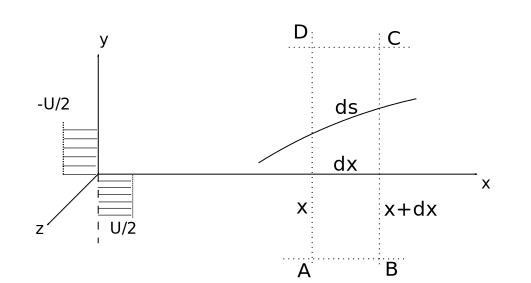
\includegraphics{../img/BR_vortex_sheet.pdf}
\caption{Vortex sheet}
\end{figure}
Let $\kappa$ be the circulation per unit length of the vortex sheet. The sheet is slightly perturbed. The rectangle ABCD contains the segment $ds$ of the sheet and the width of the rectangle is $dx$ and is equal to the projection of $ds$ on the x-axis. The circulation around the rectangle is given as,
\begin{align*}
\Gamma &=\oint \vec{u}\cdot\vec{dl} \\
\kappa ds &= \frac{1}{2}Udx+(-\frac{1}{2}U)(-dx) \\
\kappa ds &= Udx \\
\kappa &= U\frac{dx}{ds}
\end{align*}
In view of this, the B-R equations become,
\begin{subequations}\label{eq:vel_3}
\begin{equation}
u= -\oint_0^{\lambda} \frac{U}{2\lambda} \frac{\sinh k(y_1-y)}{\cosh k(y_1-y)-\cos k(x_1-x)} dx
\end{equation}
\begin{equation}
v= \oint_0^{\lambda} \frac{U}{2\lambda} \frac{\sin k(x_1-x)}{\cosh k(y_1-y)-\cos k(x_1-x)} dx
\end{equation}
\end{subequations}

This is the form we shall use for our numerical discretization. If we assume the sheet to be made up of N panels of equal length $\Delta x=\lambda/N$, then the integrals can be approximated using the rectangle rule. Denoting the strength of each point vortex as $\gamma_j (=U\lambda/N)$, we have,

\begin{subequations}\label{eq:vel_4}
\begin{equation}
u= -\sum_{j=1}^{N} \frac{\gamma_j}{2\lambda} \frac{\sinh k(y_1-y_j)}{\cosh k(y_1-y_j)-\cos k(x_1-x_j)}
\end{equation}
\begin{equation}
v= \sum_{j=1}^{N} \frac{\gamma_j}{2\lambda} \frac{\sin k(x_1-x_j)}{\cosh k(y_1-y_j)-\cos k(x_1-x_j)}
\end{equation}
\end{subequations}

If the point of interest $z_1=x_1+iy_1$ is one the point vortices, then to get the principal value of the integral, we can omit the contribution of that vortex from the summation. So the velocity induced at a point vortex $z_i=x_i+iy_i$ is given as,

\begin{subequations}\label{eq:vel_num}
\begin{equation}
u_i= \frac{dx_i}{dt}=-\sum_{\substack{j=1 \\ j\neq i}}^{N} \frac{\gamma_j}{2\lambda} \frac{\sinh k(y_i-y_j)}{\cosh k(y_i-y_j)-\cos k(x_i-x_j)}
\end{equation}
\begin{equation}
v_i= \frac{dy_i}{dt}= \sum_{\substack{j=1 \\ j\neq i}}^{N} \frac{\gamma_j}{2\lambda} \frac{\sin k(x_i-x_j)}{\cosh k(y_i-y_j)-\cos k(x_i-x_j)}
\end{equation}
\end{subequations}

It is customary to use the complex notation with $z_i=x_i+iy_i$. Hence the Equations \eqref{eq:vel_num} can be written in compact form as,
\begin{equation}\label{eq:vel_num_complex}
\frac{dz_i}{dt}=\sum\limits_{\substack{j=1 \\ j\neq i}}^{N(t)}\left(\frac{\gamma_j}{2\lambda}\right)
\frac{-\sinh{Y_{ij}}+i\, \sin{X_{ij}}}{\cosh{Y_{ij}}-\cos{X_{ij}}}
\end{equation}

where $z_i=x_i+i\,y_i, \, X_{ij}=k(x_i-x_j), \, Y_{ij}=k(y_i-y_j)$ and $k=2\pi/\lambda$.

\subsection{Issues with the formulation} 
There are two primary issues associated with the vortex sheet problem. 
\begin{itemize}
\item[1.] The short wavelength spurious growth associated with Kelvin - Helmholtz (K-H) instability
\item[2.] The failure of rectangle rule approximation when the curvature becomes comparable with vortex spacing
\end{itemize}

\subsubsection*{Resolution of Issue 1: } 
The more the number of vortices, the better approximation we get for the shape of the vortex sheet. But it is well known that the shorter wavelengths grow faster with time in K-H instability of the vortex sheet. So the errors introduced at the position of vortices during numerical calculation perturb the sheet with a wavelength equal to the spacing between vortices. Thus using more number of vortices will lead to waves growing even faster. Hence the need for using high precision arithmetic for calculations with large number of vortices. 

\subsubsection*{Resolution of Issue 2: }
Note that the summation in Equation \eqref{eq:vel_num_complex} is resulting from the use of rectangle rule for the integration in Equation \eqref{eq:vel_2}. The approximation will work well as long as the derivatives of the integrands are not too large, i.e., as long as $|\frac{dk}{ds}|,|\frac{\partial x}{\partial s}|,|\frac{\partial y}{\partial s}|$ are bounded by some constant C which is small compared to $\frac{1}{\Delta x}$ where $\Delta x$ is the spacing between vortices. To quote from Chorin and Bernard \cite{Chorin}, ``When this condition is not satisfied, the approximate balance between the flow due to the vortices on either side of a given vortex will no longer hold because of the unduly large flow produced by a point vortex, and the several vortices will capture each other, i.e., start following complicated paths around each other. Once this process starts at any point, it rapidly spreads throughout the sheet".

Though reducing $\Delta x$ seems like fixing the issue, it runs into the difficulty mentioned in Issue 1. Instead, some form of smoothing of the integrand is employed. Following Krasny \cite{Krasny}, if the point vortices are treated as blobs of radius $\epsilon$ within which they behave like a forced vortex, the current problem is resolved. The equations \eqref{eq:vel_num_complex} are modified as,
\begin{equation}\label{eq:vel_num_complex_1}
\frac{dz_i}{dt}=\sum\limits_{\substack{j=1 \\ j\neq i}}^{N(t)}\left(\frac{\gamma_j}{2\lambda}\right)
\frac{-\sinh{Y_{ij}}+i\, \sin{X_{ij}}}{\cosh{Y_{ij}}-\cos{X_{ij}}+\delta ^2}
\end{equation}
where $\delta = \epsilon / \lambda$.

Another implication of the usage of rectangle rule is that we need not use higher order methods for solving the ODE \eqref{eq:vel_num_complex_1} since we have already committed an error of order $\Delta x$.

\section{Conserved Quantities}
The desigularized Birkhoff-Rott equations as given in Equation \eqref{eq:vel_num_complex_1} are,
\begin{subequations}
\begin{equation*}
u_i= \frac{dx_i}{dt}=-\sum_{\substack{j=1 \\ j\neq i}}^{N} \frac{\gamma_j}{2\lambda} \frac{\sinh k(y_i-y_j)}{\cosh k(y_i-y_j)-\cos k(x_i-x_j)+\delta^2}
\end{equation*}
\begin{equation*}
v_i= \frac{dy_i}{dt}= \sum_{\substack{j=1 \\ j\neq i}}^{N} \frac{\gamma_j}{2\lambda} \frac{\sin k(x_i-x_j)}{\cosh k(y_i-y_j)-\cos k(x_i-x_j)+\delta^2}
\end{equation*}
\end{subequations}
Non-dimensionalizing the variables with the length scale $\lambda$ and velocity scale $U=N\gamma/\lambda$, we have,

\begin{equation}
\bar{x_i}=x_i / \lambda, \quad \bar{y_i}=y_i / \lambda, \quad \bar{t}=N\gamma t/\lambda^2, \quad %\bar{H}=H/\gamma_i^2
\end{equation}
This leads to,
\begin{subequations}\label{eq:vel_num_non_dim}
\begin{equation}
\bar{u}_i= \frac{d\bar{x}_i}{d\bar{t}}=-\frac{1}{N\gamma}\sum_{\substack{j=1 \\ j\neq i}}^{N} \frac{\gamma_j}{2} \frac{\sinh 2\pi(\bar{y}_i-\bar{y}_j)}{\cosh 2\pi(\bar{y}_i-\bar{y}_j)-\cos 2\pi(\bar{x}_i-\bar{x}_j)+\delta^2}
\end{equation}
\begin{equation}
\bar{v}_i= \frac{d\bar{y}_i}{d\bar{t}}= \frac{1}{N\gamma}\sum_{\substack{j=1 \\ j\neq i}}^{N} \frac{\gamma_j}{2} \frac{\sin 2\pi(\bar{x}_i-\bar{x}_j)}{\cosh 2\pi(\bar{y}_i-\bar{y}_j)-\cos 2\pi(\bar{x}_i-\bar{x}_j)+\delta^2}
\end{equation}
\end{subequations}

In what follows, we will leave out the overbar on the non-dimensional quantities for simplicity. The above equations \eqref{eq:vel_num_non_dim} can be written in Hamiltonian form in the following way. Let us define,
\begin{equation}\label{eq:Hamiltonian}
H=\frac{-1}{4\pi N \gamma^2}\sum_{i=1}^N\sum_{\substack{j=1 \\ j\neq i}}^{N}\gamma_i \gamma_j \log \left( \cosh {2\pi(y_i-y_j)} -\cos {2\pi(x_i-x_j)} +\delta^2\right)
\end{equation}

It is easy to check then that Equations \eqref{eq:vel_num_complex_1} can be rewritten as,
\begin{equation}\label{eq:Hamilitonian_system}
\frac{dx_i}{dt}=\frac{\partial H}{\partial y_i}\, ; \quad \frac{dy_i}{dt}=-\frac{\partial H}{\partial x_i}
\end{equation}

For example,
\begin{align*}
\frac{\partial H}{\partial y_i} &= \frac{\partial}{\partial y_i}\left(\frac{-1}{4\pi N \gamma^2}\sum_{i=1}^N\sum_{\substack{j=1 \\ j\neq i}}^{N}\gamma_i \gamma_j \log \left( \cosh {2\pi(y_i-y_j)} -\cos {2\pi(x_i-x_j)} +\delta^2\right) \right) \\
&= \frac{-1}{4\pi N \gamma^2} \times \gamma_i \sum_{\substack{j=1 \\ j\neq i}}^{N}\gamma_j\frac{\partial}{\partial y_i}\log \left( \cosh {2\pi(y_i-y_j)} -\cos {2\pi(x_i-x_j)} +\delta^2\right) \\
&= \frac{-1}{4\pi N \gamma} \sum_{\substack{j=1 \\ j\neq i}}^{N}\gamma_j\frac{\sinh 2\pi(y_i-y_j)}{\cosh 2\pi(y_i-y_j)-\cos 2\pi(x_i-x_j)+\delta^2} \times {2\pi} \\
&=  \frac{-1}{N \gamma}\sum_{\substack{j=1 \\ j\neq i}}^{N}\left(\frac{\gamma_j}{2}\right)\frac{\sinh 2\pi(y_i-y_j)}{\cosh 2\pi(y_i-y_j)-\cos 2\pi(x_i-x_j)+\delta^2} \\
&= \frac{dx_i}{dt}
\end{align*}


Since Equation \eqref{eq:Hamilitonian_system} form a Hamiltonian system, the Hamiltonian given by Equation \eqref{eq:Hamiltonian} is automatically conserved during the evolution of the vortex sheet. For numerical simulation purpose, a check on the following function will suffice for the conservation of Hamiltonian.

\begin{equation}
E=\sum_{i=1}^N\sum_{\substack{j=1 \\ j\neq i}}^{N}\log \left( \cosh {2\pi(y_i-y_j)} -\cos {2\pi(x_i-x_j)} +\delta^2\right)
\end{equation}


\section{Numerical Integration}

The Birkhoff-Rott equations are,
\begin{equation*}
\frac{dz_i}{dt}=\sum\limits_{\substack{j=1 \\ j\neq i}}^{N(t)}\left(\frac{\gamma_j}{2\lambda}\right)
\frac{-\sinh{Y_{ij}}+i\, \sin{X_{ij}}}{\cosh{Y_{ij}}-\cos{X_{ij}}+\delta ^2}
\end{equation*}
where $z_i=x_i+i\,y_i, \, X_{ij}=k(x_i-x_j), \, Y_{ij}=k(y_i-y_j), \, k=2\pi/\lambda$ and $\delta = \epsilon / \lambda$.

These are N ordinary differential equations for the complex variables $z_i$, $i=1,2,3,..N$. They must be integrated in time to get the evolution of the vortex sheet. Two approaches for solving this system is presented here. An explicit Runge-Kutta method and a semi-implicit leap-frogging approach.

\subsection{Explicit Integration}
Let us rewrite the B-R equations as an equation governing the vector $\vec{z}$ where $\vec{z}=\lbrace z_1,z_2,..z_n\rbrace$ and $z_i=x_i+i\,y_i$. i.e.,
\begin{equation}
\frac{d\vec{z}}{dt}=\vec{f}(\vec{z})
\end{equation}
Note that time does not explicitly appear in the function $\vec{f}(\vec{z})$. Let $\overrightarrow{z}^n$ be the position of vortices at time $t^n$ and $\overrightarrow{z}^{n+1}$ be the position at $t^{n+1}=t^n+\Delta t$. Then the fourth order Runge-Kutta method (RK4) gives,


\begin{align*}
\overrightarrow{k_1}&=\Delta t \times\vec{f}\left(\overrightarrow{z}^n\right) \\
\overrightarrow{k_2}&=\Delta t \times\vec{f}\left(\overrightarrow{z}^n+\frac{1}{2}\overrightarrow{k_1}\right) \\
\overrightarrow{k_3}&=\Delta t \times\vec{f}\left(\overrightarrow{z}^n+\frac{1}{2}\overrightarrow{k_2}\right) \\
\overrightarrow{k_4}&=\Delta t \times\vec{f}\left(\overrightarrow{z}^n+\overrightarrow{k_3}\right)
\end{align*}
\begin{align}
\overrightarrow{z}^{n+1}&=\overrightarrow{z}^n+\frac{1}{6}\left(\overrightarrow{k_1}+2\overrightarrow{k_2}+2\overrightarrow{k_3}+\overrightarrow{k_4}\right)
\end{align}
There are four function evaluations of $\vec{f}$ which is computationally expensive. Also we need to make sure that the time step is small enough since this is an explicit method. 

\subsection{Semi-Implicit Integration}














%\section{References}
%\begin{itemize}
%\item Krasny, R. 1986 Desingularization of periodic vortex sheet roll-up, {\it J. Comp. Phys.} {\bf 65}, p.292-313. 
%\item Abid, M., Verga ,A. 2011 Turbulence driven by singularities in vortex sheet dynamics, {\it Phys. Rev. E} {\bf 84}, 026318.
%\item Rosenhead, L. 1931 The formation of vortices from a surface of discontinuity, {\it Proc. R. Soc. London Ser. A} {\bf 134}, 823.
%\end{itemize}
\newpage
\begin{thebibliography}{99}
\bibitem{Rosenhead} Rosenhead, L. (1931) The formation of vortices from a surface of discontinuity, \emph{Proc. R. Soc. London Ser. A}, {\bf 134}, 823.
\bibitem{Abid} Abid, M., Verga ,A. (2011) Turbulence driven by singularities in vortex sheet dynamics, \emph{Phys. Rev. E}, {\bf 84}, 026318.
\bibitem{Krasny} Krasny, R. (1986) Desingularization of periodic vortex sheet roll-up, \emph{J. Comp. Phys.}, {\bf 65}, p.292-313. 
\bibitem{Chorin} Chorin, A.J. and Bernard, P.S. (1973) Discretization of a vortex sheet, with an example of roll-up, \emph{J. Comp. Phys.}, {\bf 13}, 423.
\end{thebibliography}


\end{document}